\documentclass{mcmthesis}
\mcmsetup{CTeX = false,   % 使用 CTeX 套装时, 设置为 true
        tcn = 2115481, problem = A,
        sheet = true, titleinsheet = true, keywordsinsheet = true,
        titlepage = false, abstract = true}
% \usepackage[UTF8]{ctex}
\usepackage{newtxtext}%\usepackage{palatino}
\usepackage{lipsum}
\usepackage{amsmath}
\usepackage{cite}
\usepackage{url}
\usepackage{float}
\usepackage{graphicx}
\usepackage{subfigure}
\usepackage[nottoc,notlot,notlof]{tocbibind}
\title{MCM Thesis}
\begin{document}
\begin{abstract}
  
  Fungi play a prominent role in terrestrial ecosystems, and they influence almost every aspect of terrestrial ecosystem functioning. They are the dominant decomposers of woody fibers, with direct impact on global carbon and nutrient dynamics.

  There are several factors affecting fungal decomposition. To simplify the model without loss of generality, we sort traits by Spearson correlation. The growth rate of fungus and fungus' moisture tolerance have highest correlations, thus chosen to be main factors. In Single-factor Regression Model, we evaluate how they affect the decomposition process in the presence of multiple species. With decomposition data under 10, 16, and 22 $^\circ C$, we compute linear relationships between hyphal extension rate, tolerance index and decomposition rate. Then, we build Multi-factors Regression Model using multiple linear regression algorithm, for the sake of describing how different factor combinations have influence on the decomposition rate. 
  
  Considering the interactions between multiple species, we introduce Fungal Competition Model. Starting from simplest situation, we build a model on two species with different strength. Through changing relative intrinsic rates of two, we get replacement, partial replacement and deadlock relationships. All three cases have been verified in actual experimental data. To generalize to actual situation, next we introduce multi-species competition model. Compared to former algorithm, nonlinear model works on this problem, and result shows there is periodic oscillation solution to this equation but no equilibrium point. Regarding the changing atmospheric trends, we also take soil and climate factors into consideration on the basis of former model. To visually observe the evolution of the community, cellular automata has been utilized to simulate this process.
  
  After that, we use Fungal Combination Model to predict advantages and disadvantages for species or combinations in several scenarios. Based on the cellular automata before, we get prediction curve of 3 species, 10 species and one without climate change as reference. At last, we use Simpson Index to measure the biodiversity, and predict how it has impact on overall efficiency in the Diversity of Fungal Communities Model.
  
  What's more, in the sensitivity analysis, we focus on temperature and moisture's variation range, in order to analyze their impacts on community density. Finally, we write an article for an introductory biology textbook, to discuss how people understand the ecological role of fungi these years. 

\begin{keywords}
  Fungus Community; Decomposition Process; Carbon Cycle
\end{keywords}
\end{abstract}
\maketitle
%% Generate the Table of Contents, if it's needed.
\tableofcontents
\newpage
%% Generate the Memorandum, if it's needed.
% \memoto{\LaTeX{}studio}
% \memofrom{Liam Huang}
% \memosubject{Happy \TeX{}ing!}
% \memodate{\today}
% % \logo{\LARGE I'm pretending to be a LOGO!}
% \begin{memo}[Memorandum]
%   \lipsum[1-3]
% \end{memo}

\section{Introduction}
\subsection{Problem Background}

The carbon cycle process is a very vital component of the planet. Part of the carbon cycle process is the decomposition of compounds, allowing carbon to be renewed and used in other forms. A key part of the decomposition of compounds comes from the decomposition of plant material and woody fibers. Some of the key agents in decomposing woody fibers are fungi. Studies have shown that among the many fungi traits, the growth rate of the fungus and the fungus' tolerance to moisture is the growth rate of the fungus and the fungus' tolerance to moisture. There are interesting correlations between fungi traits. And when different types of fungi coexist, they will affect each other. 

\begin{figure}[H]
\small
\centering
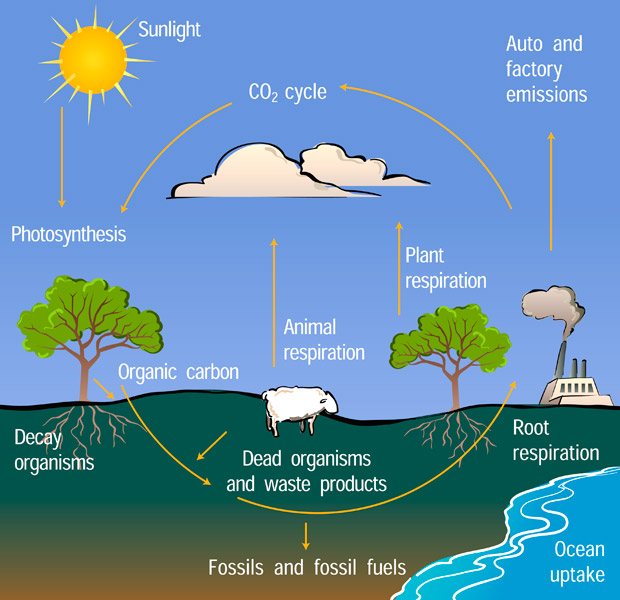
\includegraphics[width=8cm]{carbon_cycle}
\caption{A simple diagram of parts of the carbon cycle, emphasizing the terrestrial (land-based) parts of the cycle.\cite{carbon_cycle}}
\label{carbon_cycle}
\end{figure}

Thus, our team is working to better understand the relationship between traits and the competitive role of different types of fungi coexisting. In addition, it is necessary to consider the possible long-term or short-term effects of various external conditions such as different climates, seasonal changes, sudden weather, etc. 

There are many models for analyzing the relationship between various traits, such as time series, linear regression and so on. Fungi have their relatively suitable temperature, and they are sensitive to the external environment, so the model needs to be robust. For studying how the diversity of fungal communities of a system impacts the overall efficiency of a system, there are methods such as cellular automata for simulation. 

This article studies these effects, based on our proposed model, we make predictions about the relative advantages and disadvantages for each species and combinations of species likely to persist and we realize the importance and the role of biodiversity in the presence of different degrees of variability in the local environment.

\subsection{Restatement of the Problem}

Based on the relevant conclusions in the research article given in the question, our paper should continue to explore and address the following aspects. 

\begin{itemize}
  \item \textbf{Problem 1:}
  Describe the breakdown of ground litter and woody fibers through fungal activity in the presence of multiple species of fungi.
  \item \textbf{Problem 2:}
  Incorporate the interactions between different species of fungi, which have different growth rates and different moisture tolerances.
  \item \textbf{Problem 3:}
  Describe the interactions between the different types of fungi. The dynamics of the interactions should be characterized and described including both short- and long-term trends. The sensitivity to rapid fluctuations in the environment should be examined and we have to determine the overall impact of changing atmospheric trends to assess the impact of variation of local weather patterns.
  \item \textbf{Problem 4:}
  Include predictions about the relative advantages and disadvantages for each species and combinations of species likely to persist, and do so for different environments.
  \item \textbf{Problem 5:}
  Describe how the diversity of fungal communities of a system impacts the overall efficiency of a system with respect to the breakdown of ground litter. Predict the importance and role of biodiversity in the presence of different degrees of variability in the local environment.
\end{itemize}

\subsection{Our Approach}

As the question requires us, our primary goal is to model the decomposition of woody fibers in a given patch of land, and do so in the presence of multiple types of fungi breaking down woody fibers in the same area.

We consider using a linear regression model to analyze the relationship between different traits (mainly focus on the growth rate of the fungus and the fungus' tolerance to moisture and temperature) of fungi, and their impact on the breakdown of ground litter and woody fibers. Since fungus are sensitive to external environment, and considering rapid fluctuations in the environment, we specially select a robust regression algorithm: Theil-Sen Regression. According to our evaluation, it performs much better than least squares method when outliers exist.

Since the growth rate of fungi and the tolerance to moisture need to be considered comprehensively, we integrate this in our model. The relationship between fungal decomposition rate, growth rate and moisture tolerance is obtained by using multiple linear regression algorithm. 

At the same time, we consider that usually different kinds of fungi coexist, and there is a competitive relationship between them. In the end, there may only be one kind of different kinds of fungi that will survive to the end. we describe the interactions between the different types of fungi and establish a competition model, using cellular automata model to simulate the results of competition.

To predict relative advantages and disadvantages for each species and combinations of species likely to persist, we combine models above. By changing the related parameters of temperature and moisture to simulate different environmental conditions, the dual-population competition model is extended to multiple groups, and the cellular automata algorithm is used to simulate the growth of multiple groups of fungi within a certain range. Then we consider the impact of short-term and long-term climate change, and further describe the long-term trend of fungal population changes with climate. 

To describe how the diversity of fungal communities of a system impacts the overall efficiency of a system with respect to the breakdown of ground litter, we analyse biodiversity of community with Simpson index and the distribution of species in different degrees in the same local environment.

\section{Preparation of the Models}

\subsection{Assumptions and Justifications}

By adequate analysis of the problem, to simplify our model, we make the following well-justified assumptions.

\begin{itemize}
  \item There are no natural enemies in the environment where the fungus lives. The survival of fungi is only affected by the natural environment and other fungal populations.
  \item The amount of ground litter and woody fibers is limited. When there are multiple fungal populations, there may be competition for resources.
  \item In the decomposition process of ground litter and woody fibers, the intermediate stage of decomposition is the same as other stages.
  \item Environmental conditions change within an acceptable range, and there will be no continuous and destructive extreme weather.
\end{itemize}

\subsection{Notations}

For convenience, we introduce some notations below.

\begin{table}[htb]
  \centering
  \caption{Notations}
  \begin{center}
    \begin{tabular}{cc}
      \toprule[1.5pt]
      \makebox[0.3\textwidth][c]{Symbols} & \makebox[0.4\textwidth][c]{Descriptions} \\
      \midrule[1pt]
      $M$ & Mass (mg) \\
      $t$ & Time (day) \\
      $d$ & Decomposition rate (\% mass loss over 122 days) \\
      $\rho$ & Spearman rank-order correlation coefficient \\
      $ex$ & Extension rate (mm/day) \\
      $mo$ & Moisture index ($\in [-1, 1]$) \\
      $e(n)$ & Regression error \\
      $\varepsilon_p$ & Mean square of the error \\
      $a_p(k)$ & Linear regression coefficient \\
      $D_c$ & The Simpson index of area $c$ \\
      $P_i$ & Probability of species $i$ in the sample \\
      \bottomrule[1.5pt]
    \end{tabular}
  \end{center}
\end{table}

\section{Problem 1: Single-factor Regression Model}

\subsection{Feature Selection}

In the decomposition process of ground litter and woody fibers, there are usually many kinds of fungi that work together. The quantification of the decomposition process can be described by the decomposition rate $ d $. For dead branches and leaves with a mass of $ M $, the total mass may change after the time $ t $. At any moment, its decomposition rate can be expressed as: 

\begin{equation}
  d=\frac{\delta M}{\delta t}
\end{equation}

For a given piece of land, the decomposition rate of fungi varies with the various traits of different types of fungi. In order to get the change trend of the decomposition rate and each trait first, we temporarily ignore the specific value and convert the original value into a sorted label to describe the corresponding size relationship. According to the data set, for each trait $ x $ and decomposition rate $ y $, the Spearman coefficient $ \rho $ is calculated, the algorithm is as follows: 

\begin{equation}
  \rho=\frac{\sum_{i}\left(x_{i}-\bar{x}\right)\left(y_{i}-\bar{y}\right)}{\sqrt{\sum_{i}\left(x_{i}-\bar{x}\right)^{2} \sum_{i}\left(y_{i}-\bar{y}\right)^{2}}}
\end{equation}

We sort the calculation results corresponding to each trait according to the Spearman coefficient. 

\begin{figure}[H]
  \small
  \centering
  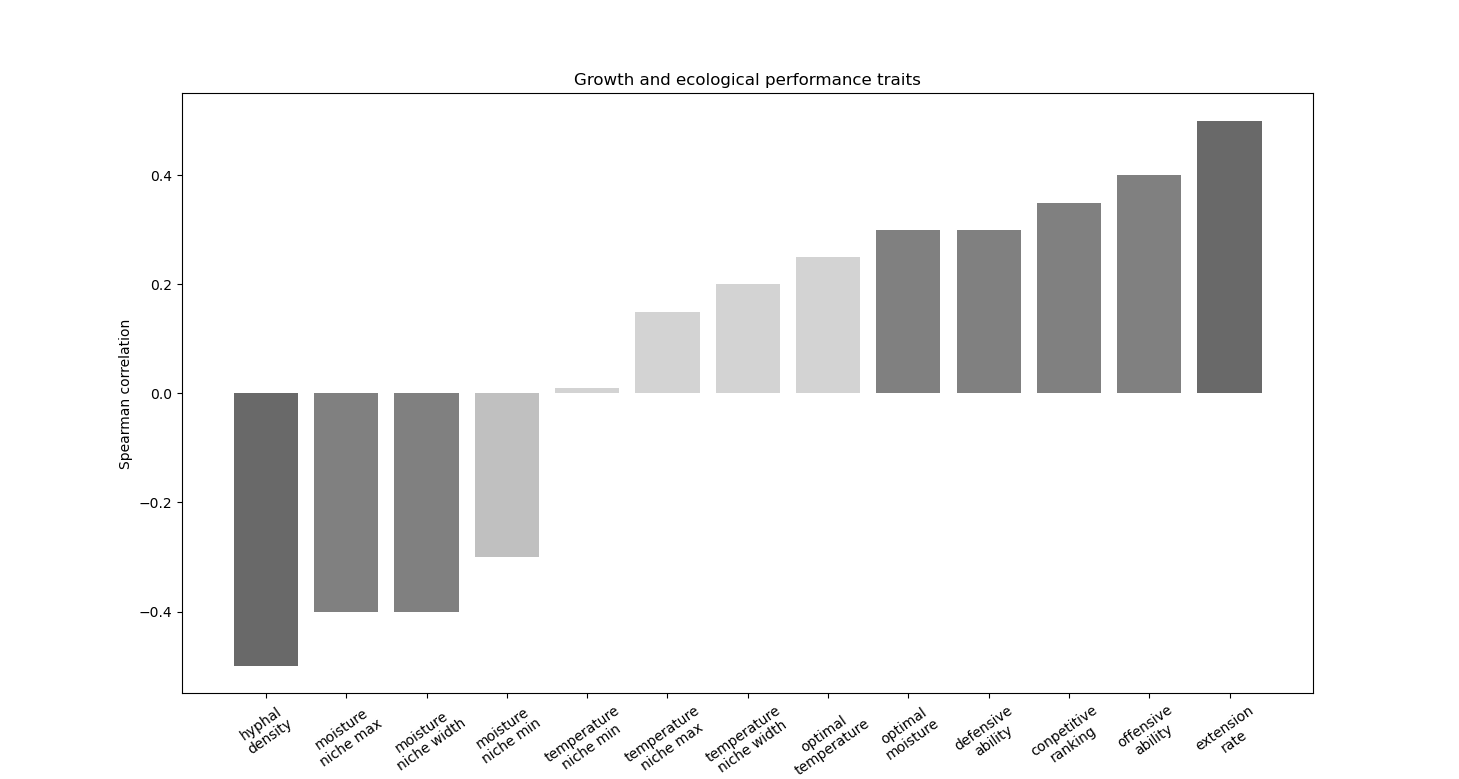
\includegraphics[width=12cm]{growth_eco_traits}
  \caption{The spearman correlation of different growth and ecological performance traits.}
  \label{growth_eco_traits}
\end{figure}

The results show that the growth rate and moisture tolerance of fungi are closely related to the decomposition process. 

Below, based on the decomposition data of 34 species of single fungus populations collected under the condition of coexistence of multiple fungi, we will regression and predict the decomposition rate of fungi, focusing on the growth rate of a single type of hyphae The relationship with decomposition rate, and the relationship between the moisture resistance and decomposition rate of hyphae. 

\subsection{The Fundamentals of Linear Regression}

The basic concept of linear regression model is that the sum of squares of the difference between the actual sampling and the linear prediction sampling reaches the minimum value, that is , the approximation of the minimum mean square error can determine the unique set of predictor coefficients.\cite{cao2009linear}

In the process of model parameter estimation, the following systems is called linear predictor.

\begin{equation}
  \hat{x}(n)=\sum_{k=1}^{p} \omega_{p}(k) x(n-k)
\end{equation}

Let $\omega_{p}(k)$ be the linear predictive coefficient and $p$ is the predictive order. The prediction error function is

\begin{equation}
  e(n)=x(n)-\hat{x}(n)
\end{equation}

That is

\begin{equation}
  e(n)=x(n)-\sum_{k=1}^{p} \omega_{p}(k) x(n-k)
  \label{alg_a}
\end{equation}

Let

\begin{equation}
  a_{p}(k)=-\omega_{p}(k)
\end{equation}

Then, (\ref{alg_a}) becomes

\begin{equation}
  e(n)=x(n)+\sum_{k=1}^{p} \omega_{p}(k) x(n-k)
  \label{alg_b}
\end{equation}

The mean square of the error is $\varepsilon_{p}=\sum_{n=p}^{N}|e(n)|^{2}$. To minimize the mean square value of the error, that is, the partial derivative is zero.

\begin{equation}
  \frac{\partial \varepsilon_{p}}{\partial a_{p}(k)}=\frac{\partial \sum_{n=p}^{N}|e(n)|^{2}}{\partial a_{p}(k)}=2 \sum_{n=p}^{N}[e(n) x(n-k)]=0
  \label{alg_c}
\end{equation}

That is

\begin{equation}
  \frac{\partial \varepsilon_{p}}{\partial a_{p}(k)}=2 \sum_{n=p}^{N}[e(n) x(n-k)]=0
\end{equation}

Substituting (\ref{alg_b}) into (\ref{alg_c}), we get

\begin{equation}
  \sum_{n=p}^{N}\left\{\left[x(n)+\sum_{k=1}^{p} a_{p}(k) x(n-k)\right] x(n-k)\right\}=\sum_{n=p}^{N} x(n) \cdot x(n-k)+\sum_{k=1}^{p} a_{p}(k) \cdot \sum_{n=p}^{N}[x(n-k) \cdot x(n-k)]
  \label{alg_d}
\end{equation}

Let

\begin{equation}
  \sum_{n=p}^{N} x(n) \cdot x(n-k)+\sum_{k=1}^{p} a_{p}(k) \cdot \sum_{n=p}^{N}[x(n-k) \cdot x(n-k)]=0
\end{equation}

In the finite sampling interval, the autocorrelation function of the real field is defined as

\begin{equation}
  r_{x}(k)=\sum_{n=k}^{N} x(n) \cdot x(n-k)(k=0,1, \cdots, p)
  \label{alg_e}
\end{equation}

Substituting (\ref{alg_e}) into (\ref{alg_d}), we get

\begin{equation}
  r_{x}(k)+\sum_{k=1}^{p} a_{p}(k) r_{x}(n-k)=0
\end{equation}

That is

\begin{equation}
  \sum_{k=1}^{p} a_{p}(k) r_{x}(n-k)=-r_{x}(k)
  \label{alg_f}
\end{equation}

We represent (\ref{alg_f}) as a matrix.

\begin{equation}
  \left(\begin{array}{cccc}
  r_{x}(0) & r_{x}(1) & \cdots & r_{x}(p-1) \\
  r_{x}(1) & r_{x}(0) & \cdots & r_{x}(p-2) \\
  \vdots & \vdots & \ddots & \cdots \\
  r_{x}(p-1) & r_{x}(p-2) & \cdots & r_{x}(0)
  \end{array}\right)\left(\begin{array}{c}
  a_{p}(1) \\
  a_{p}(2) \\
  \vdots \\
  a_{p}(p)
  \end{array}\right)=-\left(\begin{array}{c}
  r_{x}(1) \\
  r_{x}(2) \\
  \vdots \\
  r_{x}(p)
  \end{array}\right)
\end{equation}

\subsection{Decomposition Rate and Moisture Relationship}

We normalize the size of the optimal moisture range of fungus as the abscissa, $ \text {mo}=\frac{2 \times \text {width }}{\text {maxwidth }}-1 $. The zero point is the center, -1 means the fungus has the strongest moisture adaptability, and 1 means the fungus has the narrowest suitable moisture range. Plotting a scatter plot shows that the moisture resistance and decomposition rate are negatively correlated. Combining the decomposition rate of various fungi with different moisture adaptability under the same experimental conditions, using one-variable linear regression, the linear equation obtained is 

\begin{equation}
  \log {d}=1.00mo+1.74,R^2=0.3981
\end{equation}

That is

\begin{equation}
  {d}=10 ^{1.00mo+1.74}
\end{equation}

It indicates that the greater the $mo $, the worse the adaptability of the fungus and the greater the decomposition rate. It also shows that the ability of fungi to adapt to moisture is negatively related to the decomposition rate. 

\begin{figure}[H]
  \small
  \centering
  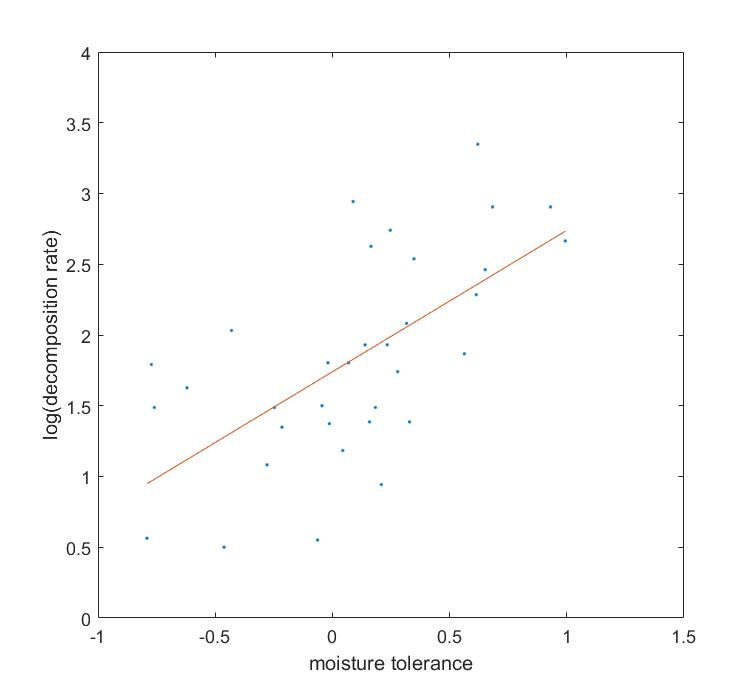
\includegraphics[width=8cm]{decomposition_moisture}
  \caption{The relationship between the moisture tolerance of various fungi and the resulting wood decomposition rate.}
  \label{decomposition_moisture}
\end{figure}

\subsection{Decomposition Rate and Extension Rate Relationship}

Then we control the moisture to remain unchanged. Taking into account the influence of temperature on the decomposition rate,  We perform linear fitting on the deposition rate and the hyphal extension rate under $ T=10, 16, 22^{\circ}C $ respectively. We get the following results. 

\begin{figure}[H]
  \small
  \centering
  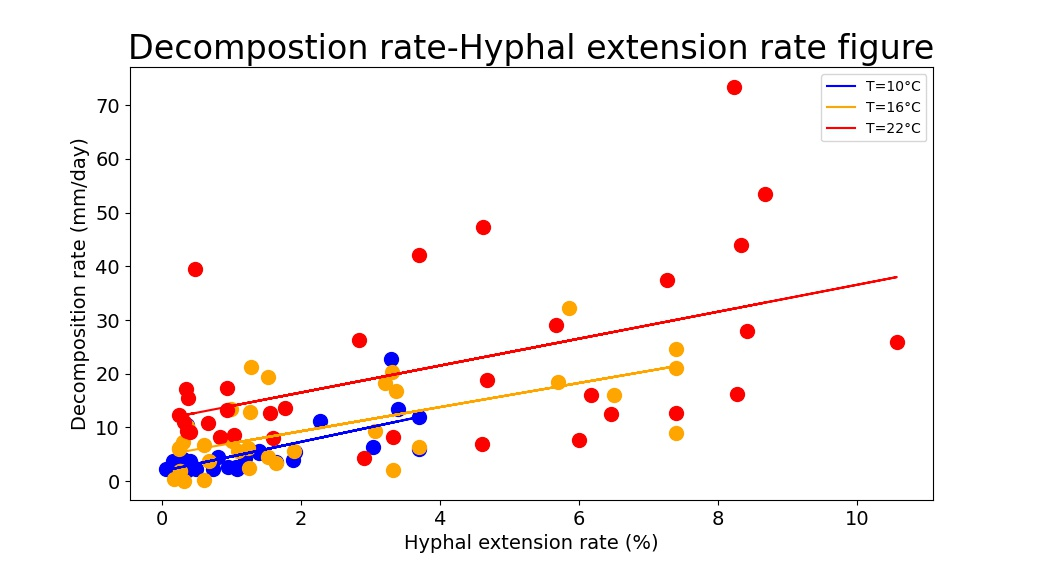
\includegraphics[width=12cm]{decomposition-extension_tot}
  \caption{The relationship between the hyphal extension rate (mm/day) of various fungi and the resulting wood decomposition rate (\% mass loss over 122 days) at various temperatures. \cite{lustenhouwer2020trait} According to the data given in the article's appendix, we re-mapped.}
  \label{decomposition-extension_tot}
\end{figure}

The corresponding equations and their correlation coefficients are: 

\begin{equation}
  \begin{split}
    d&=2.73ex+1.86,R^2=0.5009 (T=10^{\circ}C) \\
    d&=2.25ex+4.80,R^2=0.4147 (T=16^{\circ}C) \\
    d&=2.51ex+11.48,R^2=0.2511 (T=22^{\circ}C)
  \end{split}
\end{equation}

The correlation coefficient $ R^{2} $ of the linear regression model is not high. And as the temperature rises, $ R^{2} $ decreases, indicating that in a warmer soil environment, the actual relationship is more complicated than linear association. However, the model has sufficiently reflected that the decomposition rate is negatively correlated with moisture resistance. And there is a positive correlation with its extension rate.

\section{Multi-factor Regression Model}

\subsection{Problem Analysis}

In different climates, the decomposition rate of fungi is different. Even in areas with the same climate, with the changes in soil temperature, moisture and other factors, there are big differences between different parts of the fungus selected. This difference is caused by the mutual influence and interaction of many factors. Relying solely on the control variables to study the influence of certain factors on the decomposition rate is not enough to reflect the actual situation. 

According to the conclusion in question 1, the decomposition rate of ground litter and woody fibers by fungi is mainly related to the growth rate and moisture resistance of fungi. In order to comprehensively consider the influence of the two factors, we need to merge the two relationships in question 1. 

We assume that fungal growth rate and moisture tolerance are two intrinsic traits that are independent of each other. On the basis of the unary linear model in question 1, we build a multiple linear regression model. 

\subsection{Incorporate the Interactions}

Consider the situation at $16 ^ \circ C $. First, control the decomposition rate $ y $ in Model 1 unchanged. We calculate the corresponding extension rate $ x_0 $ and moisture tolerance $ x_1 $ at this time. Take some points $ (y,x_0,x_1) $ as shown in the following table: 

\begin{table}[htb]
  \centering
  \caption{Decomposition rate and extension rate and moisture relationship}
  \begin{center}
    \begin{tabular}{ccccccc}
      \toprule[1.5pt]
      \makebox[0.1\textwidth][c]{Parameter} & \makebox[0.1\textwidth][c]{Point 1} & \makebox[0.1\textwidth][c]{Point 2} & \makebox[0.1\textwidth][c]{Point 3} & \makebox[0.1\textwidth][c]{Point 4} & \makebox[0.1\textwidth][c]{Point 5} & \makebox[0.1\textwidth][c]{Point 6}\\
      \midrule[1pt]
      $y$ & 5 & 10 & 20 & 30 & 40 & 50 \\
      $x_0$ & -1.04 & -0.74 & -0.44 & -0.26 & -0.14 & -0.04 \\
      $x_1$ & 0.09 & 2.31 & 3.20 & 3.64 & 4.09 & 20.09 \\
      \bottomrule[1.5pt]
    \end{tabular}
  \end{center}
\end{table}

We assume that the decomposition rate $ Y $, the growth rate $ x_0 $ and the humidity resistance $ x_1 $ satisfy the following linear relationship: 

\begin{equation}
  Y(x)=h_\theta(x)=\theta^{\top} x=\theta_{0} x_{0}+\theta_{1} x_{1}
\end{equation}

Where

\begin{equation}
  \boldsymbol{Y}=\left(\begin{array}{c}
  y_{1} \\
  y_{2} \\
  \vdots \\
  y_{n}
  \end{array}\right), \boldsymbol{X}=\left(\begin{array}{cccc}
  1 & x_{11} & \cdots & x_{1 p} \\
  1 & x_{21} & \cdots & a_{2 p} \\
  \vdots & \vdots & \ddots & \vdots \\
  1 & x_{n 1} & \cdots & a_{n p}
  \end{array}\right), \boldsymbol{\theta}=\left(\begin{array}{c}
  \theta_{0} \\
  \theta_{1} \\
  \vdots \\
  \theta_{p}
  \end{array}\right), \boldsymbol{\varepsilon}=\left(\begin{array}{c}
  \varepsilon_{1} \\
  \varepsilon_{2} \\
  \vdots \\
  \varepsilon_{n}
  \end{array}\right)
\end{equation}

Introduce a cost function to measure the regression effect:

\begin{equation}
  J\left(\theta_{0}, \theta_{1}\right)=\frac{1}{2 m} \sum_{i=1}^{m}\left(h_{\theta}\left(x^{(i)}\right)-y^{(i)}\right)^{2}
\end{equation}

To apply the gradient descent method to our previous linear regression problem, the key is to find the derivative of the cost function, namely: 

\begin{equation}
  \frac{\partial}{\partial \theta_{j}} J\left(\theta_{0}, \theta_{1}\right)=\frac{\partial}{\partial \theta_{j}} \frac{1}{2 m} \sum_{i=1}^{m}\left(h_{\theta}\left(x^{(i)}\right)-y^{(i)}\right)
\end{equation}

When $ j=0 $:

\begin{equation}
  \frac{\partial}{\partial \theta_{0}} J\left(\theta_{0}, \theta_{1}\right)=\frac{1}{m} \sum_{i=1}^{m}\left(h_{\theta}\left(x^{(i)}\right)-y^{(i)}\right)
\end{equation}

When $ j=1 $:

\begin{equation}
  \quad \frac{\partial}{\partial \theta_{1}} J\left(\theta_{0}, \theta_{1}\right)=\frac{1}{m} \sum_{i=1}^{m}\left(\left(h_{\theta}\left(x^{(i)}\right)-y^{(i)}\right) \cdot x^{(i)}\right)
\end{equation}

Then iterate the following formulas

\begin{equation}
  \begin{split}
    \begin{array}{l}
      \theta_{0}:=\theta_{0}-a \frac{1}{m} \sum_{i=1}^{m}\left(h_{\theta}\left(x^{(i)}\right)-y^{(i)}\right) \\
      \theta_{1}:=\theta_{1}-a \frac{1}{m} \sum_{i=1}^{m}\left(\left(h_{\theta}\left(x^{(i)}\right)-y^{(i)}\right) \cdot x^{(i)}\right)
    \end{array}
  \end{split}
\end{equation}

Substitute each group of observations in the above table to estimate the regression coefficient by least squares. Regression solving the above algorithm, the regression equation is $ Y = 35.129x_0 +0.667x_1 + 37.692 $. That is $ d = 35.129ex +0.667mo + 37.692 $.

The regression plane in the three-dimensional space is shown in the figure below.

\begin{figure}[H]
  \small
  \centering
  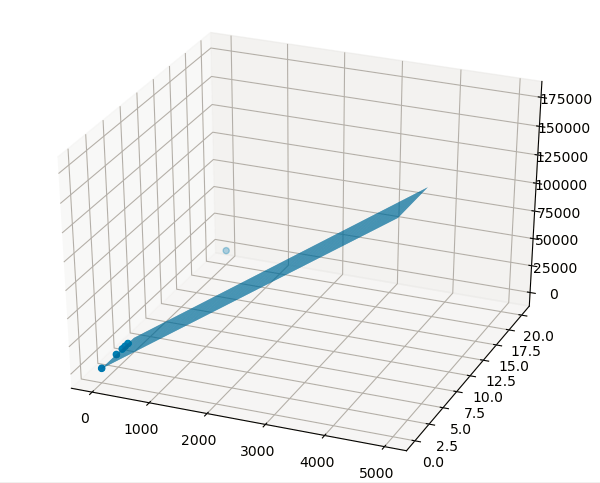
\includegraphics[width=10cm]{3dim_de_extension_moi}
  \caption{Relationship between fungi decomposition rate and growth rate and moisture tolerance.}
  \label{3dim_de_extension_moi}
\end{figure}

The result is $ \theta_0\ne0,\theta_1\ne 0 $, indicating that the regression model is effective.

\section{Fungal Competition Model}

\subsection{Interactions Between the Different Types of Fungi}

There are interactions among the various fungal populations that exist on the same ground litter and woody fibers. According to the relationship between fungi populations, fungi with different viability may have different relationships, and the establishment of these relationships often takes a certain amount of time. Therefore, in different time periods, the populations may show different interactions.

In order to simplify the problem, we simply discuss the interaction between populations. We temporarily ignore the impact of environmental changes on population relationships, and discuss according to different population abundance and initial spatial distribution. 

\begin{figure}[H]
  \small
  \centering
  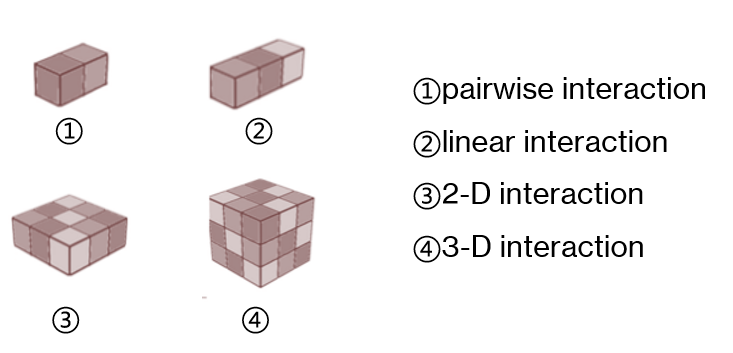
\includegraphics[width=12cm]{order_analysis_model}
  \caption{Order of analysis of our model below. The figure is drawn with \cite{hiscox2018fungus} as a reference.}
  \label{order_analysis_model}
\end{figure}

\subsubsection{Dual Population}

First, consider two populations $ x_1 $ and $ x_2 $, assuming that their number changes obey the logistic law when they live alone. We use a population competition model here.

\begin{equation}
  \left\{ \begin{array}{l} \frac{\mathrm{d} x_1}{\mathrm{d} t}=r_{1} x_1\left(1-\frac{x_1}{n_{1}}-s_{1} \frac{x_2}{n_{2}}\right)\\ \frac{\mathrm{d} x_2}{\mathrm{d} t}=r_{2} x_2\left(1-\frac{x_2}{n_{2}}-s_{2} \frac{x_1}{n_{1}}\right) \end{array} \right.
  \label{alg_31}
\end{equation}

Among them, $ x_1(t), x_2(t) $ are the numbers of the two groups A and B respectively. $ r_1, r_2 $ are their inherent growth rates, and $ n_1, n_2 $ are their maximum capacities. In terms of resources, the consumption of the unit quantity of B (relative to $n_2$) is the consumption of unit quantity A (relative to $n_1$) of $s_1$ times, and the same is true for $s_2$. 

Below we will select different model parameters to solve the model. Assume that the initial numbers of the two groups are equal, both are 120 units. 

Case 1: Set the model parameters as: 

\begin{equation}
  \left\{\begin{array}{l}
    r_{1}=0.1, \frac{1}{N_{1}}=0.002, a_{1}=0.0001 \\
    r_{2}=0.3, \frac{1}{N_{2}}=0.003, a_{2}=0.0002 \\
    x_{1}(0)=120, x_{2}(0)=120
    \end{array}\right.
  \label{alg_32}
\end{equation}

The calculation result is shown in the left diagram below.

\begin{figure}[H]
  \centering
  \subfigure
  {
    \begin{minipage}[b]{.4\linewidth}
      \centering
      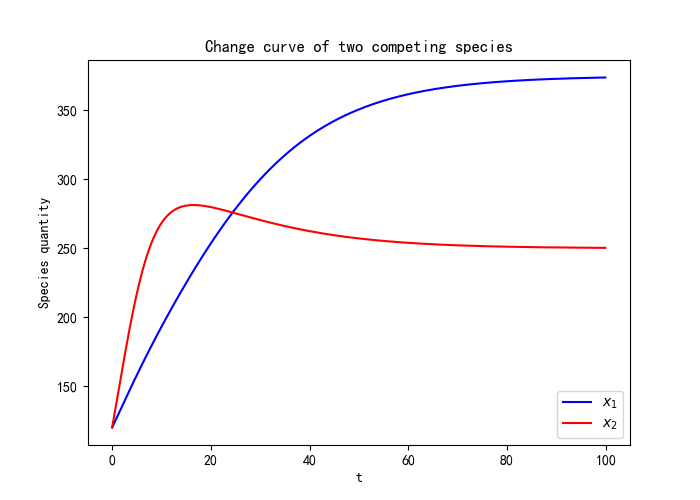
\includegraphics[scale=0.3]{curve_competing_species}
      \caption{The prediction curve of competing species}
    \end{minipage}
  }\quad \quad \quad \quad \quad \quad
  \subfigure
  {
    \begin{minipage}[b]{.4\linewidth}
      \centering
      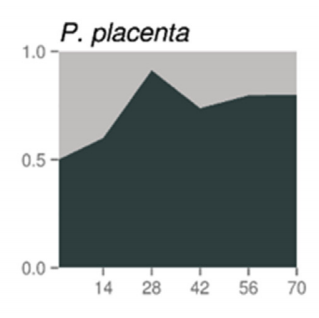
\includegraphics[scale=0.5]{amount_trametes}
      \caption{The amounts of Trametes versicolor and P. placenta}
    \end{minipage}
  }
\end{figure}

Both populations showed an upward trend after entering the group. With the consumption of resources, $ x_1 $ showed an advantage in the competition and continued to rise, while the amount of $ x_2 $ fell after reaching the peak, and both reached Stable state, but there are niche differences. According to the actual data of the researchers, there is a similar relationship between Trametes versicolor and P. placenta. The horizontal axis represents time (per day), and the vertical axis represents ratio in the community. The dark part at the bottom of the image is the proportion of P. placenta, and the light part at the top is of Trametes versicolor. The sum of the two is always 1 (the same in other cases in the following). As can be seen from the picture on the right, the ratio of the two was equal when they first entered the community, but after a period of fluctuation, the community reached a relatively balanced state. Compared with the beginning, Trametes versicolor was partially replaced.

Case 2: Set the model parameters as: 

\begin{equation}
  \left\{\begin{array}{l}
    r_{1}=0.2, \frac{1}{N_{1}}=0.002, a_{1}=0.0005 \\
    r_{2}=0.3, \frac{1}{N_{2}}=0.003, a_{2}=0.0002 \\
    x_{1}(0)=120, x_{2}(0)=120
    \end{array}\right.
  \label{alg_33}
\end{equation}

The viability of the two populations differs extremely. $ x_1 $ only rises for just a moment after entering the group, and then decreases until it is completely replaced. In other words, $ x_2 $ is eliminated by $ x_1 $. According to the actual data of the researchers\cite{hiscox2018fungus}, there is a similar relationship between Trametes versicolor and G. trabeum. Trametes versicolor is the dominant species in the competition.

\begin{figure}[H]
  \centering
  \subfigure
  {
    \begin{minipage}[b]{.4\linewidth}
      \centering
      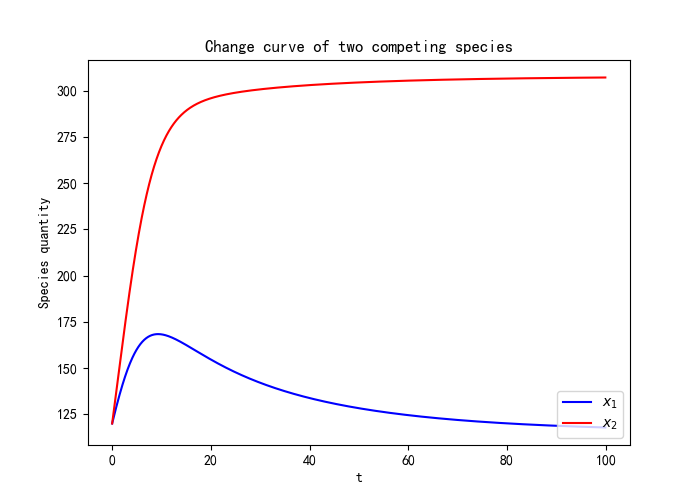
\includegraphics[scale=0.3]{curve_competing_species2}
      \caption{The prediction curve of competing species}
    \end{minipage}
  }\quad \quad \quad \quad \quad \quad
  \subfigure
  {
    \begin{minipage}[b]{.4\linewidth}
      \centering
      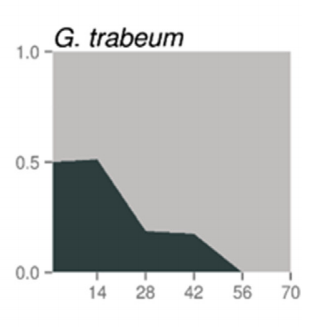
\includegraphics[scale=0.5]{amount_trametes2}
      \caption{The amounts of Trametes versicolor and G. trabeum}
    \end{minipage}
  }
\end{figure}

Case 3: Set the model parameters as: 

\begin{equation}
  \left\{\begin{array}{l}
    r_{1}=0.2, \frac{1}{N_{1}}=0.003, a_{1}=0.0002 \\
    r_{2}=0.3, \frac{1}{N_{2}}=0.003, a_{2}=0.0002 \\
    x_{1}(0)=120, x_{2}(0)=120
    \end{array}\right.
  \label{alg_34}
\end{equation}

The two populations are evenly matched and have equal strength in competition. Trametes versicolor and B. adusta have a similar relationship, the community is always relatively balanced, and two species occupy resources equally. We also say that a deadlock relationship is formed between populations.

\begin{figure}[H]
  \centering
  \subfigure
  {
    \begin{minipage}[b]{.4\linewidth}
      \centering
      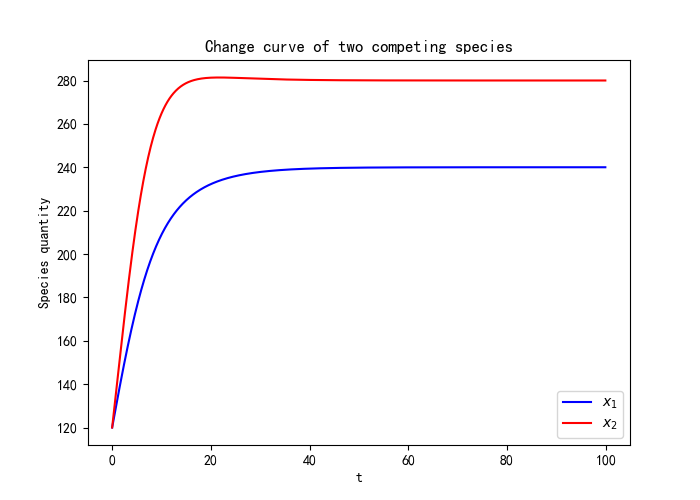
\includegraphics[scale=0.3]{curve_competing_species3}
      \caption{The prediction curve of competing species}
    \end{minipage}
  }\quad \quad \quad \quad \quad \quad
  \subfigure
  {
    \begin{minipage}[b]{.4\linewidth}
      \centering
      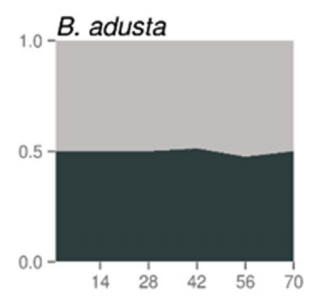
\includegraphics[scale=0.5]{amount_trametes3}
      \caption{The amounts of Trametes versicolor and B. adusta}
    \end{minipage}
  }
\end{figure}

More generally, we calculate the equilibrium point for equation (\ref{alg_31}), the determining equations for (\ref{alg_31}) are:

\begin{equation}
  \left\{\begin{array}{l}
    r_{1} x_{1}\left(1-\frac{x_{1}}{N_{1}}\right)-a_{1} x_{1} x_{2}=0 \\
    r_{2} x_{2}\left(1-\frac{x_{2}}{N_{2}}\right)-a_{2} x_{1} x_{2}=0
    \end{array}\right.
\end{equation}

It has 4 solutions:

\begin{equation}
  \left\{\begin{array}{l}
    x_{1}=0 \\
    x_{2}=0
    \end{array}, \quad\left\{\begin{array}{l}
    x_{1}=0 \\
    x_{2}=N_{2}
    \end{array}, \quad\left\{\begin{array}{l}
    x_{1}=N_{1} \\
    x_{2}=0
    \end{array}, \quad\left\{\begin{array}{l}
    x_{1}=\frac{N_{1} r_{2}\left(a_{1} N_{2}-r_{1}\right)}{a_{1} a_{2} N_{1} N_{2}-r_{1} r_{2}} \\
    x_{2}=\frac{N_{2} r_{1}\left(a_{2} N_{1}-r_{2}\right)}{a_{1} a_{2} N_{1} N_{2}-r_{1} r_{2}}
    \end{array}\right.\right.\right.\right.
\end{equation}

The first three equilibrium points are ordinary equilibrium points, and the last one is non-trivial. It can be found that when the parameter is set as (\ref{alg_32}), the equation (\ref{alg_31}) finally converges to the fourth equilibrium point, which shows that the fourth equilibrium point has strong stability.

In order to analyze the global property of the equation, we draw a directional field diagram of (\ref{alg_31}) and (\ref{alg_32}), in which the green point is the equilibrium point, and the color shades represent the changing speed at this point.

\begin{figure}[H]
  \small
  \centering
  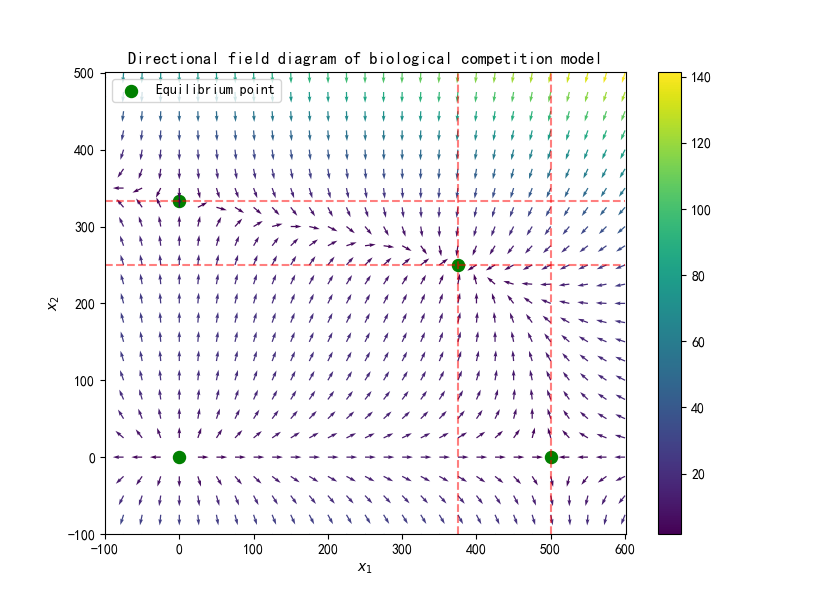
\includegraphics[width=12cm]{biological_competion_model}
  \caption{The directional field diagram of biological competition model.}
  \label{biological_competion_model}
\end{figure}

There are four equilibrium points in the diagram:

The first equilibrium point,  $ (0,0) $ at the bottom left, i.e.the case where the numbers of both species are 0, is an unstable equilibrium point. All the arrows are pointing away from the equilibrium point, which means that the tiny disturbance near the equilibrium point will eventually go far away from the equilibrium point. In other words, as long as there are a small number of species living here, they will eventually multiply and reach another equilibrium point;

The second equilibrium point,  $(0,N_2) $ at the top left, i.e. with only species  $ x_2 $ existing, belongs to the unstable equilibrium point (saddle point), and only the arrow on the vertical line past this point points to it. But all the other arrows point away from that, which means the equilibrium point is more stable than $ (0,0) $, but it is also unstable. As long as there is a small amount of species $ x_1 $, it will be far away from the current equilibrium point due to competition;

The third equilibrium point, $ (N_1,0) $ at the bottom right, is the case of only species $ x_1 $ exist, belongs to the unstable equilibrium point (saddle point). Only the arrow on the horizontal line past this point points to it. But all the other arrows move away from the equilibrium point, which means that the stability of the equilibrium point is stronger than $ (0,0) $, but it is also unstable. As long as there are a small amount of species $ x_2 $, it will be far away from the current point due to competition. 

The last equilibrium point, is $ \left(\frac{N_{1} r_{2}\left(a_{1} N_{2}-r_{1}\right)}{a_{1} a_{2} N_{1} N_{2}-r 1^{r} 2}, \frac{N_{2} r_{1}\left(a_{2} N_{1}-r_{2}\right)}{a_{1} a_{2} N_{1} N_{2}-r_{1} r_{2}}\right)$at the upper right.  Both species exist and reach a balanced state, which means a stable equilibrium point. All the arrows near the point point to it, which means that even if it deviates from the balance point to equilibrium point, it will eventually go back to the balance point.

For more clearly reflection of the flow situation at the equilibrium point, we draw the diagram of family of phase pathway (code in appendix).

\begin{figure}[H]
  \small
  \centering
  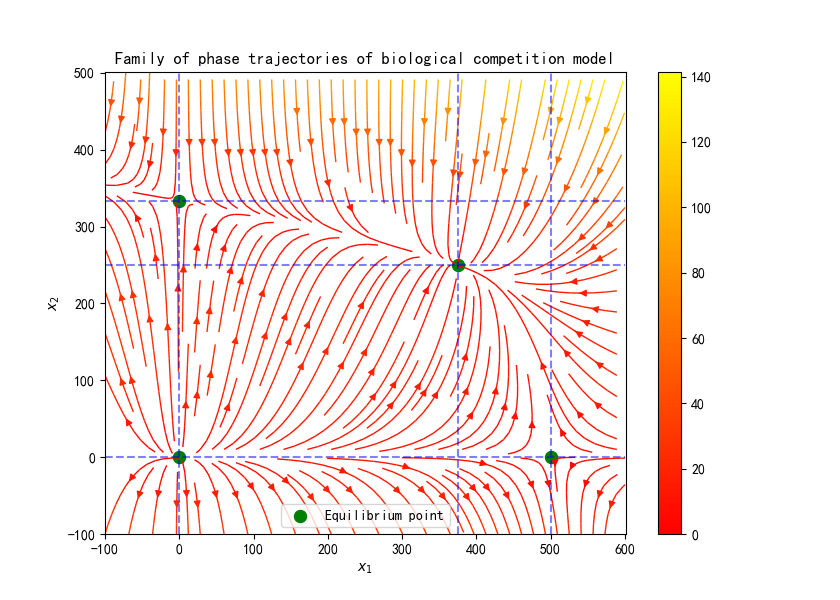
\includegraphics[width=12cm]{biological_competion_model2}
  \caption{The family of phase trajectories diagram of biological competition model.}
  \label{biological_competion_model2}
\end{figure}

In the figure, almost all the streamlines in the first quadrant (corresponding to the meaningful solution in the first quadrant) converge to the fourth equilibrium point, indicating that the fourth equilibrium point has very strong stability. This equilibrium point is The final stable point for any initial conditions.

In the phase trajectory family diagram, there is no closed phase trajectory. Therefore, the equation does not have a periodic oscillation solution.

\subsubsection{Multiple Population}

However, pairwise combinations are not always accurate predictors of outcomes of multi-species interactions, and outcomes are often less consistent in systems with multiple competitors. To accurately predict outcomes of multi-species interactions, it is significant to focus on competition between three or more species.

To simplify the model, we  introduce Gause-Lotka-Volterra (GLV) equations and considering three competitors first. The GLV equations describing the dynamics of $ n $competing populations consist of $ n $ competing populations consist of $ n $first order differential equations:

\begin{equation}
  \frac{\mathrm{d} N_{i}(t)}{\mathrm{d} t}=r_{i} N_{i}(t)\left[1-\sum_{j=1}^{n} \alpha_{i j} N_{j}(t)\right]
\end{equation}

Here $ N_{i}(t) $is the number of individuals in the $ i $th population at time $ t $, $ r_i $ is the intrinsic growth rate of the $ i $th populations, and the $ \alpha_{i,j} $are competition coefficients measuring the extent to which the $ j $th species affects the growth rate of the $ i $th.

In order to give a manageable exposition, we henceforth reduce the number of parameters in the three-competitors system by making the symmetry assumptions that (i) $ r_1=r_2=r_3=r $; (ii) with respect to competition, 2 affects 1 as 3 affects 2 as 1 affects 3, i.e., $ \alpha_{12}=\alpha_{23}=\alpha_{31}=\alpha $; (iii) similarly $ \beta_{21}=\beta_{32}=\beta_{13}=\beta $. Furthermore, we may rescale the populations $ N_i $ so that effectively $ \alpha_{ii}=1 $, and rescale $ t $ so that in effect $ r=1 $ (which embodies the assumption that $ r>0 $).

For the general case: $ \alpha + \beta > 2 $ and $ \alpha < 1 $. We now consider its solution. For definiteness we take $ \beta > 1 > \alpha $, although all the results apply, mutatis mutandis, to $ \alpha > 1 > \beta $.

At the outset, it is useful to define the positive quantity $ \gamma $:

\begin{equation}
  \gamma \equiv \alpha + \beta -2
\end{equation}

And for notation convenience we introduce $ P(t) $, the product of the three populations at time $ t $:

\begin{equation}
  P(t) \equiv N_1(t)N_2(t)N_3(t)
\end{equation}

We now get

\begin{equation}
  \frac{\mathrm{d}{\ln{P}}}{\mathrm{d}t}=-\gamma+(3+\gamma)(1-N_T)
\end{equation}

Therefore, the total time spent in the neighborhood of such a point in any one cycle is

\begin{equation}
  \begin{split}
    \tau &= \tau_{\text{in}}+\tau_{\text{out}} \\
    \tau_{\text{in}}&\simeq \frac{\gamma t}{2(\beta -1)} \\
    \tau_{\text{out}}&\simeq \frac{\gamma t}{2(1-\alpha)}
  \end{split}
\end{equation}

Thus, $ \tau $ is roughly equals

\begin{equation}
  \tau \simeq \frac{\gamma(\beta-\alpha)}{2(\beta-1)(1-\alpha)}t
\end{equation}

TODO

% ----------------

In order to make the results more intuitive, the cellular automata method is used to demonstrate below. We divide an area into many discrete points, and assume that there is at most one population on each point, and fungi can only use resources in adjacent grids. We randomly distribute several populations on the same square land, and the initial number of each population is 1.

The intrinsic growth rates of species differs greatly, which causes different distribution of species as shown below. To simplify the shape of figure, we chose 3 species as initial live species. The series below shows the distribution of species. The green cells stand for sources or nutrition, the colored turtles stand for fungal individuals.

TODO

To get more generate interaction rule between multi species, we enlarged initial species to 10, and recorded population amounts continuously. In the figure below, x-axis stands for ticks of iteration, y-axis stands for percent of living species, ans different color stands for different species.

\begin{figure}[H]
  \small
  \centering
  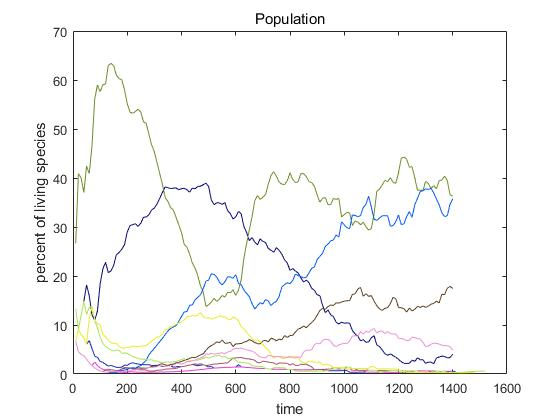
\includegraphics[width=12cm]{density_proportion}
  \caption{The change of population density proportion.}
  \label{density_proportion}
\end{figure}

In round 1400 of iteration, there are just five alive species existing on the land, with others eliminated. And species of brown and blackish green line are in the dominate position in the community. The quantity of dominant species fluctuates periodically, which confirms the previous conclusion of  Gause-Lotka-Volterra equation.

\subsection{Short- and Long-term Trends Analysis}

Considering the influence of climate factors on the long- and short-term trends of fungal growth, we make the following analyse: 

As for the short-term trend, we assume that the external environmental factors will stay the same, and the only factor affecting the competitiveness of fungi in the coexistence of multiple groups is their traits. That is to consider the fungal growth and competitiveness under the currently determined temperature and humidity. So for the short-term trend, we can regard it as the model in the previous section.

As for the long-term trend, we will consider the suitable moisture range of fungi, and investigate the influence of periodic climate change on the growth trend of fungi. It is assumed that the temperature and humidity of the environment change with a period of one year, and that the growth rate of fungi changes with a sinusoidal period, i.e. $ r_i = \frac {r_{i0} \times (2-k_i + \sin(2\pi t/365)\times k_i ) }{2} $($ k_i $ is the factor of fungi growth rate affected by moisture, which reflects the humidity tolerance of fungi). Take $ \left\{\begin{array}{l}
    r_{1}=0.2, \frac{1}{N_{1}}=0.002, a_{1}=0.0001 \\
    r_{2}=0.3, \frac{1}{N_{2}}=0.002, a_{2}=0.0002 \\
    x_{1}(0)=120, x_{2}(0)=120
    \end{array}\right. $to the equation (\ref{alg_31}), consider the periodic change of $ r_i $,  the population change curves with $ \left\{\begin{array}{l}
    k_{1}=1 \\
    k_{2}=1
    \end{array}\right. $ and $ \left\{\begin{array}{l}
    k_{1}=0.5 \\
    k_{2}=1
    \end{array}\right. $ are drawn respectively, as shown in the figure below. In the figure, the growth rate of $ x_1 $ is slightly lower than that of $ x_2 $, but the competitiveness is slightly better than that of $ x_2 $. the moisture tolerance of $ x_1 $and $ x_2 $ in the left figure is the same, and that of $ x_2 $in the right figure is slightly lower than $ x_1 $.

TODO

\subsection{Examination of the Sensitivity to Rapid Fluctuation}

We consider rapid fluctuation as cases including sudden rainfall, snowfall, and other conditions, that can cause sudden changes in humidity and temperature in the growing environment. The observations under such rapid fluctuation conditions will be regarded as discrete ones, which will cause error in the prediction and analysis of the long-term trend. To make some adjustments  in our regression model, we introduce the robust regression algorithm: The Huber Regression algorithm and Theil-Sen Regression algorithm, to replace the Linear regression algorithm based on the least-square method used previously.

The Huber loss is a robust loss function for regression problems defined as

\begin{equation}
  \mathcal{L}(y, \hat{y})=\left\{\begin{array}{lll}
  (y-\hat{y})^{2} & \ldots & |y-\hat{y}| \leq \alpha \\
  |y-\hat{y}| & \ldots & |y-\hat{y}|>\alpha
  \end{array}\right.
\end{equation}

Where $y$ is the target variable, $ \hat{y} $ are the corresponding predictions and $ \alpha \in \mathbb{R}^+ $ is a hyperparameter. It is tempting to look at this loss as the log-likelihood function of an underlying heavy tailed error distribution. Indeed, for absolute errors smaller than $\alpha$ the corresponding distribution resembles the normal distribution, outside this region it coincides with the more heavy-tailed Laplace distribution. This is precisely the reason why this loss is robust against outliers. \cite{huber_regression}

Another alternative to least squares for simple linear regression is Theil-Sen estimation. This more robust method determines the slope of the regression line via the median of the slopes of all lines that can be drawn through the data points:

\begin{equation}
  r_{\mathrm{TS}}(x, y)=\operatorname{sign}\left(m_{\mathrm{TS}}(y, x)\right) \cdot \sqrt{m_{\mathrm{TS}}(y, x) \cdot m_{\mathrm{TS}}(x, y)}
\end{equation}

If the median slopes have the same sign, and zero otherwise. The condition to set the measure to zero on sign change of the slopes might seem artificial. However, the median slope generically does not change sign when exchanging $x$ and y, and when it does, the Kendall rank correlation between $x$ and y vanishes.\cite{theil_sen_regression}

Take the regression of decomposition rate and extension rate at 10 $ ^\circ C $ as an example. In order to examine the sensitivity to rapid fluctuation of each algorithm, we will artificially add a number of outliers, and compare the fitting effects of various regression algorithms through graphing.

\begin{figure}[H]
  \small
  \centering
  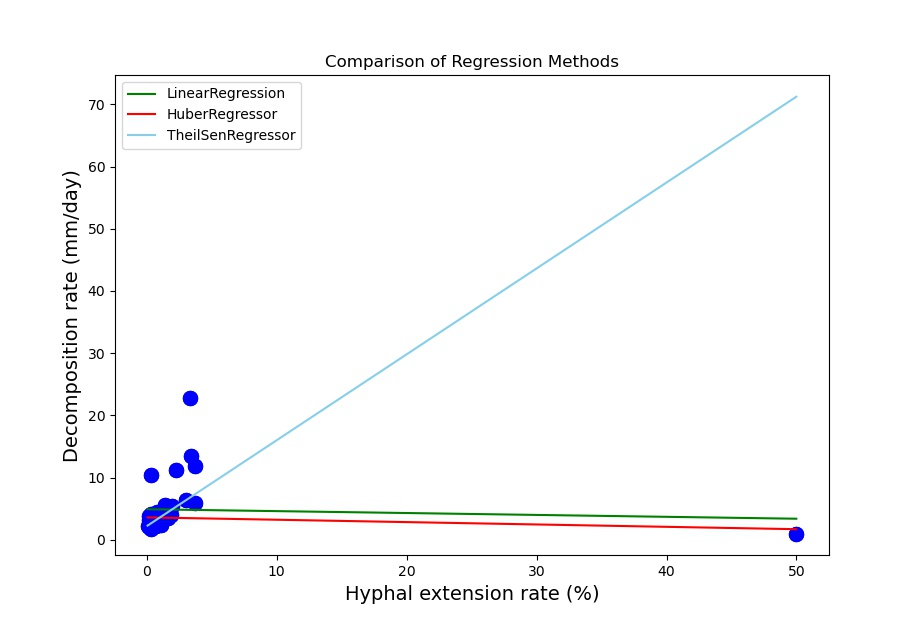
\includegraphics[width=12cm]{comparison}
  \caption{The fit of the three models after adding artificial outlier $(50, 1)$. It can be seen that Thei-Sen Regression model has outstanding performance.}
  \label{comparison}
\end{figure}

\begin{table}[htb]
  \centering
  \caption{The quantitative evaluation results of the three models, where MAE stands for Mean Absolute Error and STD stands for standard deviation. The smaller the MAE and STD, the better. }
  \begin{center}
    \begin{tabular}{ccc}
      \toprule[1.5pt]
      \makebox[0.3\textwidth][c]{Algorithm} & \makebox[0.2\textwidth][c]{MAE} & \makebox[0.2\textwidth][c]{STD} \\
      \midrule[1pt]
      Linear Regression & 6.599 & 10.851 \\
      Huber Regression & 5.147 & 7.926 \\
      Theil-Sen Regression & 3.943 & 5.885 \\
      \bottomrule[1.5pt]
    \end{tabular}
  \end{center}
\end{table}

Theil-Sen Regression model performs the best. It has a certain filtering effect on outlier, and can better present the normal development trend. Because the sudden fluctuation of external conditions can be characterized as outlier, thus, the analysis of the long-term trend that needs to filter out the sudden fluctuation of environmental factors can use the Theil-Sen Regression model to fit the previously mentioned humidity and growth rate.

\section{Problem 4:  Fungal Combinations Model}

Because the optimal temperature, moisture and other parameters of different populations are very different, and there are interactions between populations. Therefore, under different environmental conditions, stable populations, dominant populations, and the entire fungal community have very different decomposition rates for dead branches and leaves. 

\subsection{Abstract the Parameters of Different Climatic Conditions}

Here, the annual precipitation laws of different climate types are used to indicate the range of humidity changes. For example, arid areas are dry and less rainy throughout the year, with small changes in humidity, while temperate areas have obvious dry and rainy seasons with large humidity changes. We normalize the humidity change range to $[-1,1] $, $ -1 $ represents a large humidity change range, and $ 1 $ represents a small humidity change.

For regions with different climate types, temperature differences in different seasons, different weather, and different time periods are also considered. For the sake of simplifying the model, the analysis is carried out here based on the daily average temperature only in units of four seasons in a year. Among them, in order to reduce the sudden change that may be caused by the temperature difference under different weather conditions, the fitting is performed by the previously described Theil-Sen Regression algorithm with better performance.

\begin{table}[htb]
  \centering
  \caption{The quantitative evaluation results of the three models, where MAE stands for Mean Absolute Error and STD stands for standard deviation. The smaller the MAE and STD, the better. }
  \begin{center}
    \begin{tabular}{ccc}
      \toprule[1.5pt]
      \makebox[0.3\textwidth][c]{Area} & \makebox[0.3\textwidth][c]{Temperature $^\circ C$ \cite{temperature}} & \makebox[0.15\textwidth][c]{Moisture Index} \\
      \midrule[1pt]
      Arid (Tarim Basin)& [14.2, 24.4, 11.1 -4.7] & 1 \\
      Semi-arid (Bismarck) & [-8, 6, 23, 8] & 0.2 \\
      Temperate (Beijing) & [3, 22, 26, 6.5] & -1 \\
      Arboreal area & 24-28 & 0.8 \\
      Tropical rain forests (Amazon rainforest) & about 30 & 1 \\
      \bottomrule[1.5pt]
    \end{tabular}
  \end{center}
\end{table}

\subsection{Prediction of Advantages and Disadvantages in Different Environments }

The community structure varies in different climate scenarios, and its evolution relationship and changes with climate are also more complicated. Below we will use the previous cellular automata model to simulate the entire community. Three kinds of simulations are carried out under each environment. Firstly, the change trend of the three groups is simulated to reflect the evolution relationship of simple community structure; then 10 species are introduced and the observation time is extended to reflect the evolution process of more complex populations; finally, the evolution of climate change The parameters are removed from the initial state of the model as a theoretical reference.

Case 1: In arid zones, there are large temperature fluctuations, low precipitation. This requires higher tolerance for fungi, but causes lower decomposition rate relatively.

TODO

It can be seen from the figure that the stability of the community takes a long time, and populations with comparable viability are more likely to resist extreme environmental conditions. Intolerant colonies cannot join the competition or are eliminated at the beginning. After the community structure is relatively stable, there is a dynamic balance among several populations, and each population shows periodic fluctuations, but because fungi has good tolerance, the overall decomposition situation is relatively stable.

Case 2: In semi-arid area, there is periodic precipitation. Compared with the conditions in Case 1, the requirements for the moisture resistance of fungi are reduced.

TODO

Compared to arid, the environment becomes more mild for fungi, especially for competitive ones in the extension stage. As shown in the middle figure, after around 1000 rounds, more species become extinct. However, without climate change, there may be more species existing in the same patch. This reveals species with both better tolerance and dominance can survive better.

Case 3: In temperate region, resources are relatively more abundant, which can support more individuals.

TODO

As the species abundance increases, the magnitude of the number changes gradually decreases. However, at each moment, the gap between the dominant species and others is more evident. Under ideal conditions, there are more competitors existing at the same time, which reveals climate changes have played a role in natural selection.

Case 4: In arboreal, The content of humus increase, the soil has higher temperature and moisture, which can accommodate more kinds of fungi.

TODO

It can be seen from the comparison that under the same climate conditions, the change trend of the three populations and the multi populations is roughly the same. There is no absolute dominant species in the community. When there are fluctuations in the environment, there is a shift between several populations with higher niche. Species with higher extension rate in this situation are in an advanced position in the community.

Case 5: In tropical rain forests, the climate is more stable, suitable for more species of fungi. And the chemical metabolism is accelerated, ground litter and woody fibers is rich, and there is a continuous supply of nutrient in the soil.

TODO

In this case, the community composition is more complex and the dominance is reduced. After slight climate change, the ecological structure remains stable. When the C element is used as the main measurement standard, the dominant species in the figure above have a greater impact. When other elements or components are used as the measurement standard, the results may be inverted. On the whole, the community is more abundant, the dominant population is different under different standards, and the overall decomposition efficiency is high.

\section{Diversity of Fungal Communities Model}

\subsection{Diversity of Fungal Communities Simulation}

According to the experimental data\cite{maynard2019consistent}, When multiple populations coexist, it can decompose ground litter and wood fibers faster and more stably than a single population. This is due to the following reasons:

\begin{itemize}
  \item Different types of fungi have different ability to decompose chemical substances containing C, N, P and K. compared with a single population, they can decompose all parts of withered branches and leaves significantly.
  \item The decomposition of single type of fungi is mainly used to provide energy for its own growth and respiratory consumption. When there is competition between types of fungi, there will be additional energy consumption, so more energy intake is needed.
  \item Some types of fungi produced by the interaction between strains can accelerate the decomposition of plant debris.
\end{itemize}

Therefore, the combination of multiple strains can get better decomposition effect.

In order to quantify the biodiversity of fungi, Simpson index is introduced to evaluate.

For an area, we assume that this is a community $ c $, common $ S $species of fungi, $ N $individuals of fungi, The individual number of each fungus is $ N_i $, that is

\begin{equation}
  D_c=1-\sum_{i=1}^{S}\left(\frac{N_i}{N}\right)^{2}
\end{equation}

Since we can't count the number of individual fungi in the environment, we adopt the sampling method. In the sample, it is assumed that the proportion of each fungus is $ P_i $, We think that the proportion of the individual of the fungus in the environment is $ P_i $, that is

\begin{equation}
  D_c=1-\sum_{i=1}^{S}P_i^{2}
\end{equation}

Given $ S $, When there is $ P_j(1\leq{j} \leq{S})\rightarrow{1} $, there is $\lim_{P_j \rightarrow 1}{D_c}=\lim_{P_j \rightarrow 1}{\left(1-\sum_{i=1}^{S}P_i^{2}\right)}=0$.

It can be considered that there is only one species in the community, and the decomposition rate model of the community degenerates to the situation in model 1.

It can be proved that, when $ P_1=P_2=...=P_S $, Simpson index reach the maximum$ \left(1-\frac{1}{S}\right) $, At this time, all kinds of fungi coexist in the community and form a complex and stable interaction relationship. According to model 3, in areas with high temperature and moisture, there are often more combinations of populations living at the same time, $ D_c $increased, and the decomposition rate of the community increased.

At the same time, the optimal temperature and moisture of different types of fungi are also different, and the combination of multiple strains can have high decomposition rate in different weather conditions. According to the conclusion of model 4, when the environmental conditions change, the original dominant population in the combination may become a weak population, and the original weak population will become a dominant population, so the total decomposition rate does not fluctuate greatly due to the changes of environmental conditions.

We use the efficiency of carbon as the efficiency of fungi decomposing organic matter on the ground. The relationship between species richness and carbon use efficiency is obtained by statistical analysis of fungal communities with different species richness under different temperature, moisture and ground organic matter. It can be concluded that with the increase of species richness, the carbon use efficiency is on the rise, that means, the decomposition rate is increased. In multiple measurements, the higher the species richness is, the smaller the variance of carbon use efficiency is. This can represent that when the species richness is higher, the decomposition rate is more stable, and can face the complex external environmental conditions, The stable decomposition rate can be maintained when the environment changes.


\begin{figure}[H]
  \small
  \centering
  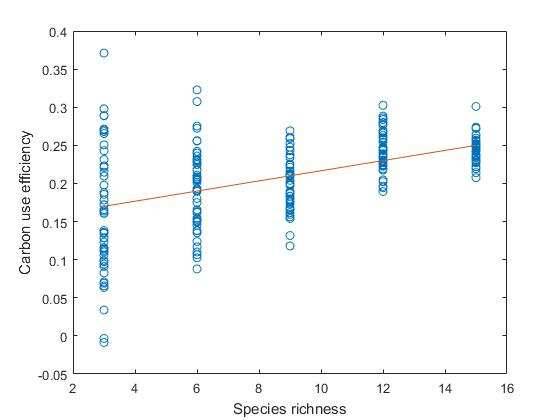
\includegraphics[width=12cm]{species_richness_carbon}
  \caption{Effects of species richness on carbon use efficiency.}
  \label{species_richness_carbon}
\end{figure}

In addition, there are great differences in different parts of the same area. For example, land use change directly influences soil microbial communities by altering vegetation cover\cite{li2019spatial}.Figures below show fungi distribution in woodland, shrubland and open area. It is shown that even in the same park, there are still evident differences between patchs. The x-axis and y-axis stand for easting and northing (meter).

TODO

Thus, tree distribution-induced shifts in local environments controlled the spatial variations in soil fungi community structure within one land use type, highlighting that the role of spatial heterogeneity in microbial communities has important implications for land management and carbon cycle.

\subsection{The Importance and Role of Biodiversity }

In the ecosystem, different organisms absorb and metabolize different substances. Multi species coexistence can make different species cooperate with each other and get what they need. Biodiversity can make the ecosystem more stable, and ecosystems with good biodiversity can withstand a wider range of environmental changes. The change of environment also makes the survival ability and competition ability of species change. The ecosystem with insufficient biodiversity may lack enough species to adapt to the environment after the change of environment, resulting in ecosystem imbalance. The ecosystem with biodiversity can adapt to the new environment by adjusting the quantity of species in the ecosystem.

\section{Sensitivity Analysis }

Through the above analysis, the symbiotic relationship of various fungi under different environmental factors is obtained, and the combination of fungi that may appear for a long time in different climates is given. Influenced by various external factors, climatic conditions may change in a certain range. Next, taking the sensitivity analysis of temperature and moisture variation range under different climatic conditions. Using the temperate climate as an example, when the average temperature and moisture of that year fluctuate within the range of 5\%, the population density change obtained is as shown in the figure below, and the change range is within 5\%, so it can be considered that the model is relatively stable.

TODO

\section{Conclusion}

\subsection{Summary of Results}

\subsubsection{Result of Problem 1}

Through the calculation of Spearman coefficient $ \rho $, it is found that the decomposition rate  is mainly related to the growth rate and humidity tolerance of fungi. By using the linear regression method, the relationship between the decomposition rate of fungi at different temperatures and the growth rate and moisture tolerance of fungi is obtained.

\begin{equation}
  \begin{split}
    \log {d}&=1.00mo+1.74,R^2=0.3981 \\
    d&=2.73ex+1.86,R^2=0.5009 (T=10^{\circ}C) \\
    d&=2.25ex+4.80,R^2=0.4147 (T=16^{\circ}C) \\
    d&=2.51ex+11.48,R^2=0.2511 (T=22^{\circ}C)
  \end{split}
\end{equation}

\subsubsection{Result of Problem 2}

In order to find out the influence of multiple factors on fungal decomposition rate, we integrate the fungal growth rate and humidity tolerance in question 1, and use multiple linear regression algorithm to obtain the relationship between fungal decomposition rate and growth rate and humidity tolerance.

$ d = 35.129ex +0.667mo + 37.692 $

\subsubsection{Result of Problem 3}

In order to explore the internal relationship between the coexistence of different fungi, a population competition model is constructed for two fungal populations to solve the differential equation, The growth law of fungi with different growth rate and different environmental adaptability in pairwise competition is described, and the phase diagram of birth and growth process is described. Then, the two population competition model is extended to multi population, and the cellular automata algorithm is used to simulate the growth of multi population fungi in a certain range. Then, the effects of short-term and long-term climate change on temperature and humidity are considered, and the long-term variation trend of fungal population with climate is further depicted.

Finally, robust region algorithm: Huber regression algorithm and Theil-Sen regression algorithm are used to test the sensitivity of fungal community to rapid environmental change. And it is concluded that the Theil Sen regression model can better filter the sudden factors in the environment, so as to better predict the long-term trend.

\subsubsection{Result of Problem 4}

The factors affecting fungal growth and inter ethnic competition are comprehensively evaluated, and the possible long-term fungal assemblages under several representative climatic conditions are predicted. After extracting the characteristics of different climatic conditions, we use cellular automata, introduce 10 species and deduce the evolution process of the population. When the population number is stable, it is the species combination that may exist for a long time under this climatic condition.

In arid zones, it takes a long time for the community to be stable, and the populations with the same survival ability are more likely to resist the extreme conditions of the environment, and the intolerant colonies can not join the competition or be eliminated at the beginning. After the community structure is relatively stable, there is a dynamic balance among several populations, and each population presents a periodic fluctuation. However, due to the good tolerance of fengi, the overall decomposition is relatively stable.

In semi-arid area, The environment becomes more mild for fungi, especially for competitive ones in the extension stage. Species with both better tolerance and dominance can survive better.

In temperate region, as the species abundance increases, the magnitude of the number changes gradually decreases. At each moment, the gap between the dominant species and others is more evident. Under ideal conditions, there are more competitors existing at the same time, which reveals climate changes have played a role in natural selection.

In arboreal,  the change trend of the three populations and the multi populations is roughly the same. There is no absolute dominant species in the community. When there is fluctuation in the environment, several populations in higher niche will change. Species with higher extension rate in this situation are in an advanced position in the community.

In tropical rain forests, The community composition is more complex and the dominance is reduced. After slight climate change, the ecological structure remains stable. On the whole, the community is more abundant, the dominant population is different under different standards, and the overall decomposition efficiency is high.

\subsubsection{Result of Problem 5}

Simpson index is used to evaluate the biodiversity of regional fungi from multiple perspectives, and the fungal species richness model is established. The results showed that with the increase of species richness, the carbon use efficiency showed an upward trend, that is, the decomposition rate increased. In multiple measurements, with the increase of species richness, the variance of carbon use efficiency decreased, which could represent the increase of carbon use efficiency when the species richness is higher The solution rate is more stable, can face the complex external environment conditions, and can maintain a stable decomposition rate when the environment changes. It can be concluded that when the environment changes, the ecosystem with biodiversity can adapt to the new environment through the adjustment of species population structure in the ecosystem.

\subsection{Strengths}

\begin{itemize}
  \item Among growth and ecological performance traits that have impact on decomposition rate, we use Spearman correlation to analyze main traits, which can greatly represent most situations.
  \item When analysing the dynamic interactions of the population, we take different cases into consideration, and introduce relative equations for precise calculation.
  \item Considering the influences of environmental factors, computer simulation is utilized for predicting the future community evolution.
\end{itemize}

\subsection{Possible Improvements}

\begin{itemize}
  \item When simulating the interaction of fungi, the simulation is performed only on a two-dimensional plane, without considering the changes of fungi in different depths of the actual soil. There are lots of work to do on 3-D simulation model.
  \item The relationships between temprature and decompotition rate only select three typical decrete values, which cannot describe all posible temperature conditions.
  \item To simplify the model, Fungal combination model take average temprature and moisture as parameters. To some extent, some continuous condition cannot be redlected, which can cause some error. In futher work, we will collect continuous data to fit the actural situations better.
\end{itemize}








\bibliography{ref}{}
\bibliographystyle{plain}

\newpage

\begin{appendices}

\section{Article}

% \begin{letter}{Dear, Mr. Alpha Chiang}

% its a letter

% \vspace{\parskip}

% Sincerely yours,

% Your friends

% \end{letter}

Carbon cycle is the most important one in the chemical cycle of the earth. Carbon exists in the form of organic matter and inorganic matter on the earth, and constantly transforms between organic matter and inorganic matter. Carbon is essential to biology and is closely related to our life. fungi play the role of decomposers in the carbon cycle. They can accelerate the speed of carbon cycle, which is conducive to the rapid progress of carbon cycle. They can decompose the remains of animals and plants and release them into carbon dioxide into the air or carbonate into the soil for plant use. Although fungi are tiny, they can decompose ground litter and woody fiber and play an important role in the carbon cycle of the ecosystem.

\begin{figure}[H]
  \small
  \centering
  
\includegraphics[width=8cm]{fungal}
  \label{fungal}
\end{figure}

We can consider that the extension rate and moisture tolerance of fungi are the main factors affecting the decomposition of ground litter and woody fiber. Through the analysis of a large number of data, using the method of linear regression, the decomposition rate of fungi is positively correlated with the extention rate of fungi, and negatively correlated with the moisture tolerance. In other words, the faster the fungi grow, the faster they can decompose, while the fungi with better moisture tolerance have a smaller decomposition rate.

\begin{figure}[H]
  \small
  \centering
  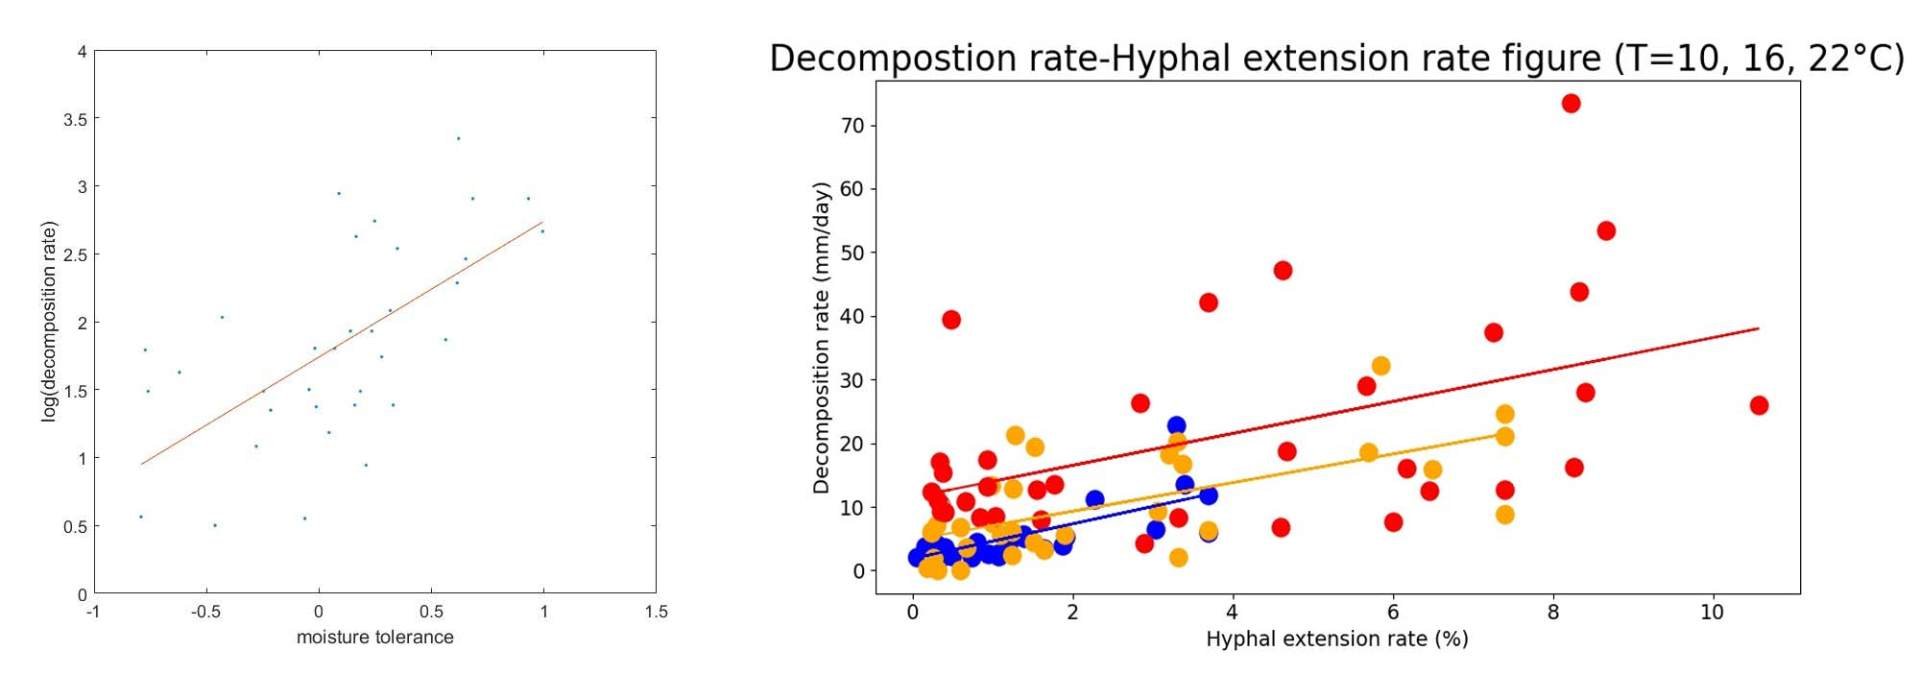
\includegraphics[width=12cm]{regression_compound}
  \label{regression_compound}
\end{figure}

In the natural environment, a certain kind of fungus usually does not exist alone, but often coexists with many kinds of fungi. We can use the population competition model to describe the growth of many kinds of fungi coexisting. The growth rate and competitiveness of each fungal population are affected by temperature and moisture. The proportion of fungal population after a period of time is obtained by cellular automata algorithm. When the time is long enough, the population of each fungi maintains a stable value, or changes with the climate change. If the climate changes with the annual cycle, the population of each fungal population also changes with the annual cycle.

TODO

\begin{figure}[H]
  \small
  \centering
  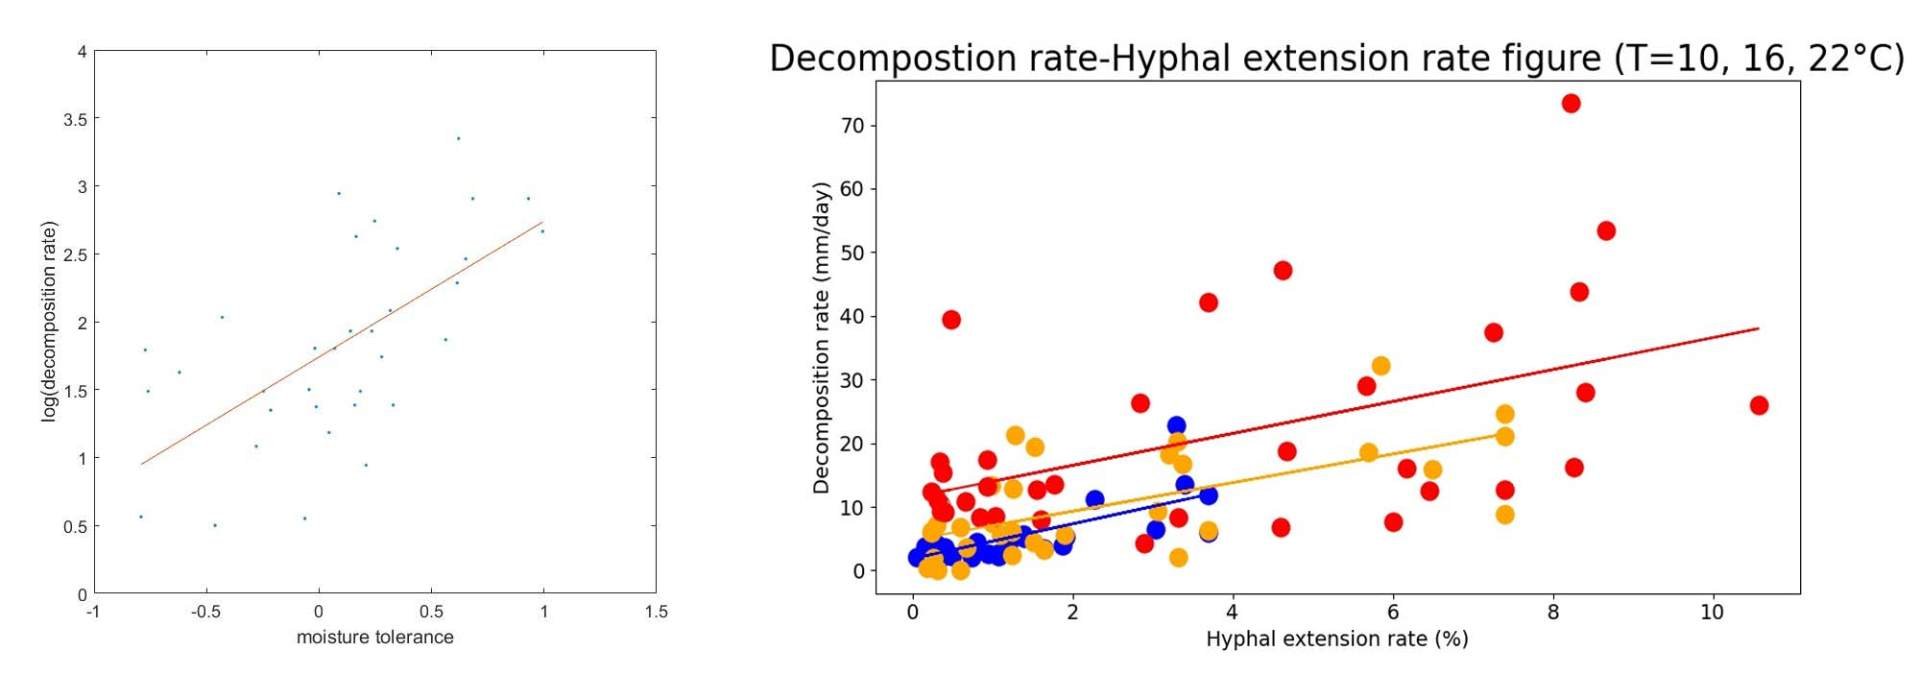
\includegraphics[width=12cm]{regression_compound}
  \label{regression_compound}
\end{figure}

In several representative climates, arid, semi-arid, temperate, arboreal, and tropical rain forests. In arid zones, there are large temperature fluctuations, low precipitation. This requires higher tolerance for fungi, but causes lower decomposition rate relatively. 

In semi-arid area, Due to the existence of periodic precipitation, compared with the conditions in arid area, the requirement of humidity tolerance of fungi decreased. The environment becomes more mild for fungi, especially for competitive ones in the extension stage. Species with both better tolerance and dominance can survive better.

In temperate region, resources are relatively more abundant, and the species abundance increases, the magnitude of the number changes gradually decreases. However, at each moment, the gap between the dominant species and others is more evident. 

In arboreal, With the increase of humus content, the soil has higher temperature and moisture, which can accommodate more kinds of fungi. There is no absolute dominant species in the community. When there are fluctuations in the environment, there is a shift between several populations with higher niche. Species with higher extension rate in this situation are in an advanced position in the community.

In tropical rain forests, the climate is more stable and suitable for more kinds of fungi. There is a continuous supply of nutrient in the soil. The community composition is more complex and the dominance is reduced. The ecological structure remains stable after slight climate change. On the whole, the community is more abundant, the dominant population is different under different standards, and the overall decomposition efficiency is high.

As we all know, fungi are usually multi-population coexistence. There is not only competition but also cooperation between different fungi. Different fungi absorb and metabolize different chemicals. They absorb their own nutrients in the same area, and it is also possible that the metabolites of one fungus are the substances that another fungus needs to absorb. Different fungi have different optimal growth conditions. When the environment changes, the fungal community of a single population may be unable to adapt to the new environment, but the population density gradually decreases, which eventually leads to the imbalance of the ecosystem. When the environment changes, the growth ability and competitiveness of species within the community will change, and the dominant species may replace, But on the whole, the total decomposition rate of all fungi did not change dramatically. Through the evaluation of biodiversity and the analysis of a large number of data, conclude that with the increase of species richness of fungal community, the total decomposition rate showed an upward trend, and the variance of total decomposition rate under different growth conditions decreased, indicating that the diversity of fungal species can help fungal community to have a higher and more stable decomposition rate when the environment changes. In nature, fungi can decompose the corpses or remains of animals and plants, and promote the material circulation in nature. The diversity of fungi can make this process stable under environmental changes, so as to maintain the balance of the ecosystem.

TODO




% \section{Programs}
% \textbf{\textcolor[rgb]{0.98,0.00,0.00}{Input Python source:}}
% \lstinputlisting[language=Python]{./code/extension_decomposition_temp.py}
\end{appendices}
\end{document}